\documentclass[a4paper, 12pt, final, garamond]{book}
\usepackage{cours-preambule}

\raggedbottom

\makeatletter
\renewcommand{\@chapapp}{Optique -- chapitre}
\makeatother

\begin{document}
\setcounter{chapter}{2}

\chapter{Correction du TD}

\section{Constructions optiques de lentilles}

Construisez les images par la lentille des objets suivants. On donnera à chaque
fois la nature de l'objet et de l'image.

\subsection{Pour une lentille convergente}
\begin{multicols}{2}
    \begin{enumerate}
        \item ~\smallbreak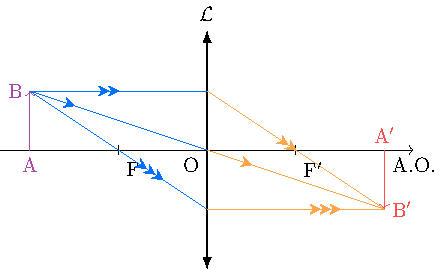
\includegraphics[width=\linewidth]{convAF}
            Ces rayons, issus d'un \underline{objet réel}, se croisent après la
        lentille : on a un faisceau émergent \underline{convergent} qui
        donne une \underline{image réelle}.
        \item ~\smallbreak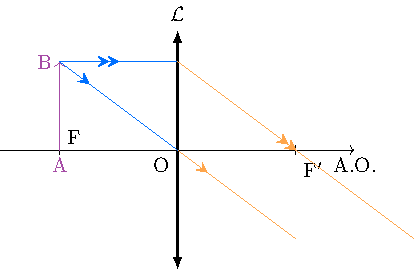
\includegraphics[width=\linewidth]{convBF}
            Ainsi, à partir d'un \underline{objet réel}, on obtient des rayons
            \underline{parallèles} qui donnent une \underline{image à l'infini}.
            \columnbreak
        \item ~\smallbreak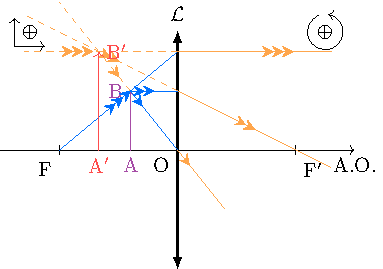
\includegraphics[width=\linewidth]{convCF}
            Ici, l'objet est \underline{réel} mais donne un faisceau émergent
            \underline{divergent}, donnant donc une image \underline{virtuelle}.
        \item ~\smallbreak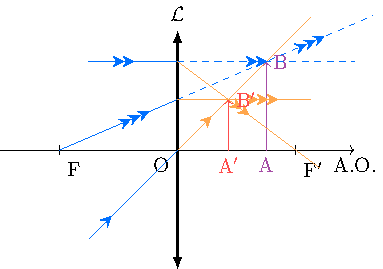
\includegraphics[width=\linewidth]{convDF}
            On part d'un \underline{objet virtuel}. Les rayons partant de la
            gauche du système passent par $B$, mais une fois arrivés à la
            lentille on continue les traits en pointillés pour montrer que ce
            sont des rayons virtuels. Le faisceau émergent est
            \underline{convergent}, donnant lieu à une \underline{image réelle}.
            \columnbreak
        \item ~\smallbreak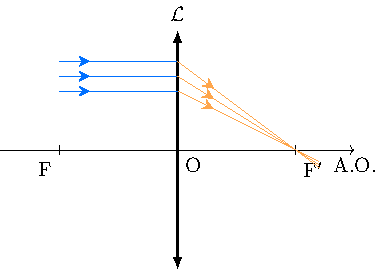
\includegraphics[width=\linewidth]{convHF}
            Ici, l'objet est \underline{réel} et donne un faisceau émergent
            \underline{convergent}, donnant donc une image \underline{réelle}.
        \item ~\smallbreak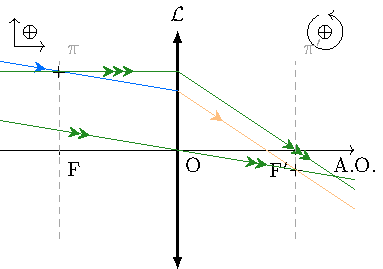
\includegraphics[width=\linewidth]{convQQE}
            On n'a qu'un seul rayon, donc pas d'intersection~: aucune idée de la
            nature de l'objet/image.
    \end{enumerate}
\end{multicols}

\subsection{Pour une lentille divergente}
\begin{multicols}{2}
    \begin{enumerate}
        \item ~\smallbreak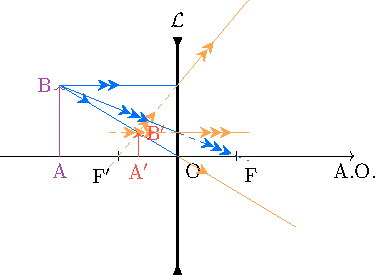
\includegraphics[width=\linewidth]{divAF}
            Ces rayons, issus d'un \underline{objet réel}, se croisent avant la
        lentille : on a un faisceau émergent \underline{divergent} qui
        donne une \underline{image virtuelle}.
        \item ~\smallbreak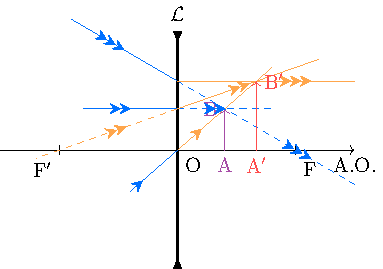
\includegraphics[width=\linewidth]{divBF}
            Ainsi, à partir d'un \underline{objet virtuel}, on obtient des rayons
            \underline{convergents} qui donnent une \underline{image réelle}.
            \columnbreak
        \item ~\smallbreak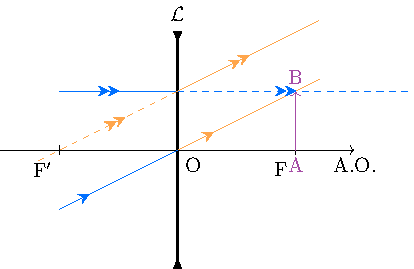
\includegraphics[width=\linewidth]{divCF}
            Ici, l'objet est \underline{virtuel} et donne un faisceau émergent
            \underline{parallèle}, donnant donc une image \underline{à l'infini}.
        \item ~\smallbreak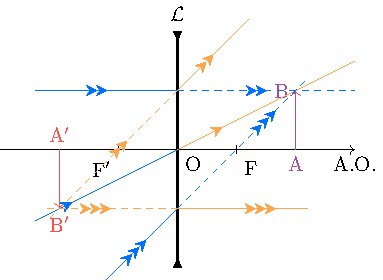
\includegraphics[width=\linewidth]{divDF}
            On part d'un \underline{objet virtuel}. Le faisceau émergent est
            \underline{divergent}, donnant lieu à une \underline{image virtuelle}.
            \columnbreak
        \item ~\smallbreak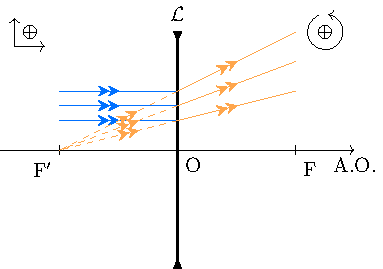
\includegraphics[width=\linewidth]{divHF}
            Ici, l'objet est \underline{réel} et donne un faisceau émergent
            \underline{divergent}, donnant donc une image \underline{virtuelle}.
        \item ~\smallbreak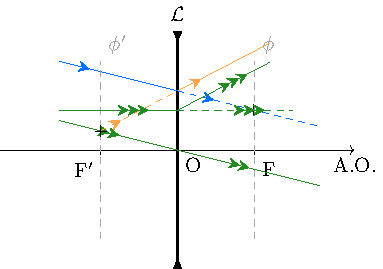
\includegraphics[width=\linewidth]{divQQE}
            On n'a qu'un seul rayon, donc pas d'intersection~: aucune idée de la
            nature de l'objet/image.
    \end{enumerate}
\end{multicols}

\section{Constructions optiques de miroirs}
\begin{NCdefi}[tabularx={Y|Y|Y}]{Schéma}
    &&\\
    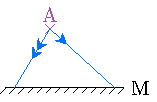
\includegraphics{td3-2-1a} &
    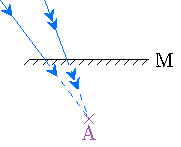
\includegraphics{td3-2-2a} &
    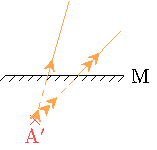
\includegraphics{td3-2-3a}\\
    Les rayons, incidents, se coupent avant le miroir. &
    Les rayons, incidents, se coupent après le miroir. &
    Les rayons, émergents, se coupent après le miroir.\\
\end{NCdefi}
\begin{tcbraster}[raster columns=2, raster equal height=rows]
    \begin{NCprop}[]{Résultat attendu}
        Construire les objets et images avec les règles du miroir plan.
    \end{NCprop}
    \begin{NCrapp}[]{Outils}
        Image par miroir plan = symétrique. Objet à intersection des indicents,
        image intersection émergents.
    \end{NCrapp}
\end{tcbraster}
\begin{NCexem}[tabularx={Y|Y|Y}]{Application}
    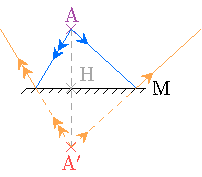
\includegraphics{td3-2-1b} &
    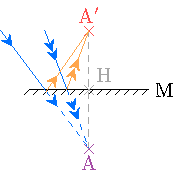
\includegraphics{td3-2-2b} &
    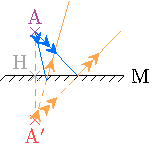
\includegraphics{td3-2-3b}\\
    Le symétrique de A donne A' où les rayons émergents se croisent. &
    Le symétrique de A donne A' où les rayons émergents se croisent. &
    Le symétrique de A' donne A où les rayons incidents se croisent.\\
    A est réel, A' virtuel. &
    A est virtuel, A' réel. &
    A est réel, A' virtuel.\\
\end{NCexem}

\section{Vidéoprojecteur}

\begin{NCdefi}[sidebyside, sidebyside align=center]{Données}
    \begin{enumerate}
        \item $(AB) = \SI{24}{mm}$ : « l'objet est une matrice de $ \SI{24}{mm}$
            » ;
        \item $ \obar{OA'} = \SI{+4.0}{m}$ : « l'écran se situe à $\SI{4.0}{m}$ »
            (c'est là que se forme l'image, c'est donc la position de $A'$) ;
        \item $ \obar{OF'} = \SI{+5.0}{cm}$.
    \end{enumerate}
    \tcblower
    \begin{center}
        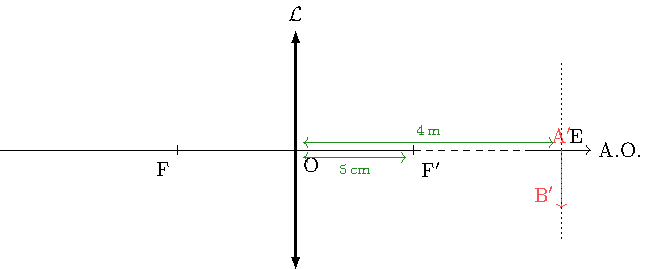
\includegraphics[width=\linewidth]{videoproj_plain.pdf}
    \end{center}
\end{NCdefi}
\begin{tcbraster}[raster columns=2, raster equal height=rows]
    \begin{NCprop}{Résultats attendus}
        \begin{enumerate}
            \item Que vaut $ \obar{OA}$ ? : « Déterminer la position et la nature de
                l'objet » ($O$ est bon point d'intérêt à partir duquel on peut
                mesurer des distances, et selon la valeur \underline{algébrique} de
                $\obar{OA}$ on saura de quel côté de la lentille l'objet se situe,
                et donc son caractère virtuel ou réel) ;
            \item Que vaut $\ABp$ ? : « Déterminer [...] la taille de l'image ».
        \end{enumerate}
    \end{NCprop}
    \begin{NCrapp}{Outils du cours}
        \begin{enumerate}
            \item Relation de conjugaison pour une lentille mince :
                \[ \boxed{ \frac{1}{\OF} = \frac{1}{\OAp} - \frac{1}{\OA}}\]
            \item Grandissement pour une lentille mince :
                \[\boxed{\g = \frac{\ABp}{\ABb} = \frac{\OAp}{\OA}}\]
        \end{enumerate}
    \end{NCrapp}
\end{tcbraster}
\begin{NCexem}[breakable, sidebyside]{Application}
    \begin{enumerate}
        \item De la relation de conjugaison, on a :
            \[\OA = \left[ \frac{1}{\OAp} - \frac{1}{\OF} \right]^{-1}\]
            Et avec les données,
            \[ \boxed{\OA = \SI{- 5.0}{cm}}\]
            Ainsi, on a un \underline{objet réel} situé à 5 centimètres à gauche de
            la lentille.

        \item De l'expression du grandissement, on a :
            \[\ABp = \ABb\times\frac{\OAp}{\OA}\]
            Et avec les données,
            \[ \boxed{\ABp = \SI{- 1.9}{m}} \]
    \end{enumerate}
    \tcblower
    \begin{center}
        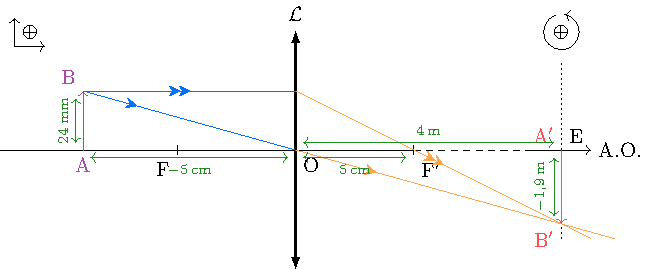
\includegraphics[width=\linewidth]{videoproj.pdf}
    \end{center}

\end{NCexem}

\begin{NCrema}{Remarque}
    Attention, comme on a qu'un seul chiffre significatif, on a $\OA =
    \SI{-5}{cm}$, ce qui semble correspondre à la position de $F$, mais en
    réalité ce n'est qu'une approximation numérique. Comme $\OAp \gg \OF$, le
    résultat numérique est proche de $-\OF$, mais il est évident que si l'objet
    était en effet au foyer objet, le vidéoprojecteur ne formerait pas l'image
    sur l'écran mais à l'infini.
\end{NCrema}

\section{Œil réduit et accommodation}
\begin{NCdefi}{Données}
    \begin{minipage}{0.5\linewidth}
        \begin{enumerate}
            \item Rétine = écran, \smallbreak
                cristallin = lentille ;
            \item Au repos, $A$ à l'infini ;
            \item Au \textit{proximum}, $A$ à \SI{25}{cm} \smallbreak
                ($\OA = \SI{-25}{cm}$).
        \end{enumerate}
    \end{minipage}
    \begin{minipage}{0.5\linewidth}
        \begin{center}
            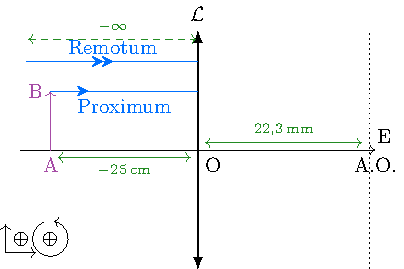
\includegraphics[width=\linewidth]{oeil_plain.pdf}
        \end{center}
    \end{minipage}
\end{NCdefi}

\begin{tcbraster}[raster columns=2, raster equal height=rows]
    \begin{NCprop}{Résultats attendus}
        \begin{enumerate}
            \item $\OF _\mathrm{repos}$ ?
            \item $\OF _\mathrm{accomodation}$ ?
        \end{enumerate}
    \end{NCprop}
    \begin{NCrapp}{Outils du cours}
        Relation de conjugaison pour une lentille mince, avec $\OAp =
        \obar{OE} = \SI{22.3}{mm}$ (le principe d'un écran c'est que l'image
        se forme dessus !!) et $\frac{1}{\OA} = 0$ quand $\OA =
        -\infty$
    \end{NCrapp}
\end{tcbraster}

\begin{NCexem}[breakable, sidebyside]{Résultats}
    \[ \boxed{\OF_\mathrm{repos} = \SI{22.3}{mm}}\]
    \begin{center}
            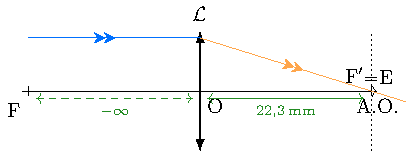
\includegraphics[width=\linewidth]{oeil_repos.pdf}
    \end{center}
    \tcblower
    \[ \boxed{\OF_\mathrm{accomodation} = \SI{20.6}{mm}} \]
    \begin{center}
            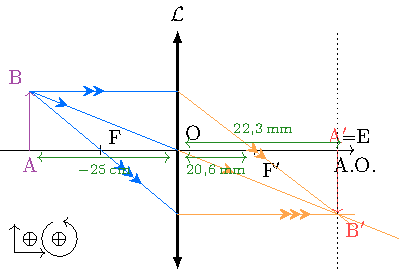
\includegraphics[width=\linewidth]{oeil_acco.pdf}
    \end{center}

\end{NCexem}

\section{Coin de miroir}
\begin{minipage}{0.48\linewidth}
    
    On compte 3 réflexions, et il doit revenir sur lui-même~: le rayon incident
    et le rayon émergent doivent faire le même angle avec la normale à $BC$.
    L'angle $i_2$ est également identique de $I$ à $J$ et de $J$ à $I$. Cela
    n'est vérifié que si la lumière est en incidence normale sur $AB$.

    Or, $i_1 = \frac{\pi}{2} - \alpha$, donc $i_2 = -i_1 =
    \alpha-\frac{\pi}{2}$. Pour avoir $i_2$ dirigé verticalement, il faut
    $-i_1+i_2 = -\frac{\pi}{2}$, autrement dit $2i_1 = \frac{\pi}{2}
    \Leftrightarrow i_1 = \frac{\pi}{4}$. Finalement, on trouve

    \begin{empheq}[box=\fbox]{equation*}
        \alpha = \frac{\pi}{4}
    \end{empheq}
\end{minipage}
\hfill
\begin{minipage}{0.48\linewidth}
    \begin{center}
        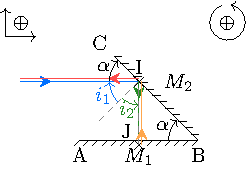
\includegraphics[width=\linewidth]{coin_mir.pdf}
        \captionof{figure}{Schéma du système}
        \label{fig:coin_mir}
    \end{center}
\end{minipage}

\section{Étude d'un rétroprojecteur}

\begin{enumerate}
    \item On a $AB \opto{\Lc}{O} A_1B_1 \opto{M}{H} A'B'$, avec $H$ le point
        d'intersection entre le miroir plan et l'axe optique de la lentille.
        L'image finale $A'$ donnée par le miroir plan est telle que
        \begin{empheq}[box=\fbox]{equation*}
            \obar{HA'} = \obar{HA_1} = D
        \end{empheq}
        On a donc pour la lentille
        \begin{empheq}[box=\fbox]{align*}
            \obar{OA_1} &= \obar{OH} + \obar{HA_1}\\
            \Leftrightarrow \obar{OA_1} &= d+D
        \end{empheq}
        On utilise la relation de conjugaison des lentilles minces en nommant
        $V$ la vergence de la lentille~:
        \begin{equation*}
            V = \frac{1}{d+D} - \frac{1}{-h} \Leftrightarrow
            \boxed{h = \frac{d+D}{V(d+D)-d}}
            \quad\text{avec}\quad
            \left\{
                \begin{array}{rcl}
                    d & = & \SI{10e-2}{m}\\
                    D & = & \SI{3.0}{m}\\
                    V & = & \SI{2.0}{m^{-1}}
                \end{array}
            \right.
        \end{equation*}
        Et l'application numérique donne
        \begin{equation*}
            \boxed{h = \SI{60}{cm}}
        \end{equation*}
    \item Le miroir plan a un grandissement de 1, donc le grandissement du
        système est celui de la lentille~: on a $\gamma = \DS
        \frac{\obar{A_1B_1}}{\obar{AB}} = \frac{\obar{OA_1}}{\obar{OA}}$, soit
        \begin{empheq}[box=\fbox]{align*}
            \gamma &= \frac{d+D}{-h}\\
            \gamma &= -5.2
        \end{empheq}
\end{enumerate}

\end{document}

